\chapter{Systemarkitektur}

%\section{Arkitektur}
% % % % %  Indleding til Arktiktur % % % % % %

For at skabe overblik over samtlige dele af systemet, udarbejdes der SysML systemarkitektur. 
SysML diagrammerne danner overblik over hele systemet og hjælper med at danne en nemmere overgang til design og implementeringsfasen. 
Systemarkitekturen er bygget op således, at jo længere frem i arkitekturen man kommer, desto flere detaljer får man for systemet. 



\clearpage
% % % % % Diagrammer med dertil beskrivelser % % % % %


\subsection{Sequence Diagram Use Case 1}

Det første diagram, der udarbejdes er Sekvens diagrammet for Use Case 1.
Sekvensdiagrammet er med til at give overblik over de forskellige funktioner, der skal implementeres i design og implementeringsfasen.
På sekvensdiagrammet tilføjes også States, som benyttes i State Machine Diagrammet, som kan ses senere i arktitekturen. 

\begin{figure}[H]
\centering
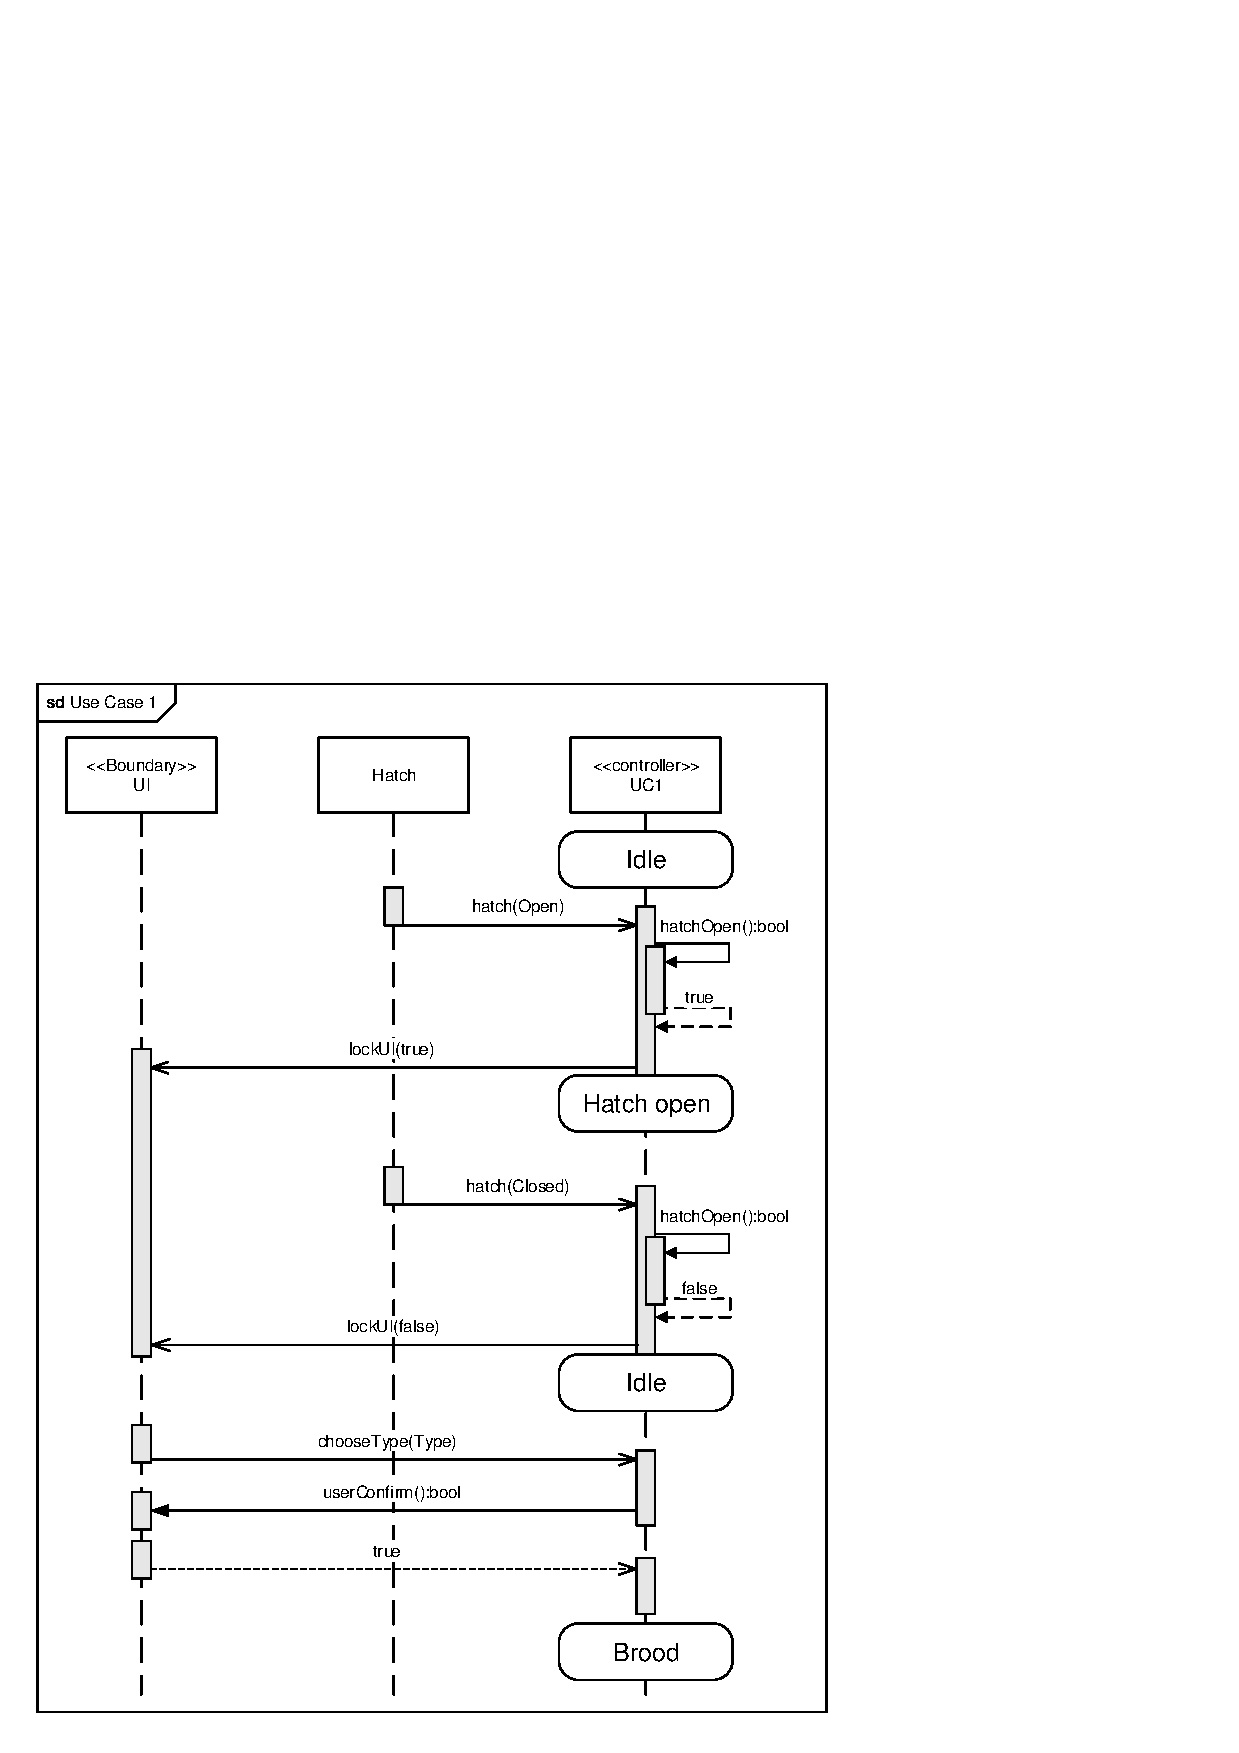
\includegraphics[page=1,width=\linewidth,viewport=07mm 08mm 139mm 180mm]{./2_systemarkitektur/diagrammer/ArkitekturDiagrammer.pdf}
\caption[Diagram]{Sequence diagram - Use Case 1}
\label{fig:SystemStateDiagram}
\end{figure}

\clearpage

\subsection{Sequence Diagram Use Case 2}

I sekvensdiagrammet nedenfor beskrives den overordnede interaktion mellem systemets dele i konteksten af Use Case 2. Systemet initierer udrugningssekvensen, hvor der kontinuert reguleres på temperatur og luftfugtighed, og hvor der tjekkes om æggene skal vendes. Når denne sekvens er afsluttet, informerer systemet brugeren om dette. Dernæst reguleres temperatur og luftluftighed indtil alle udrugede emner er fjernet fra systemet. Herefter stoppes regulering af temperatur samt luftfugtighed, og systemet går i sin idle-state.

\begin{figure}[H]
\centering
\includegraphics[page=2,width=\linewidth,viewport=8mm 265mm 268mm 573mm]{./2_systemarkitektur/diagrammer/ArkitekturDiagrammer.pdf}
\caption[Diagram]{Sequence diagram - Use Case 2}
\label{fig:SystemStateDiagram}
\end{figure}
\clearpage


\subsection{State Machine Diagram}

State Maskine diagrammet bruges til at vise de forskellige stadier systemet kan befinde sig i, samt overgang mellem dem. Systemet har fire stadier: ”Idle”, ”Brood”, ”Done” samt ”Hatch Open”.  Det blev valgt at der er mulighed for at gå til ”Idle” fra de tre andre stadier. For at have mulighed for at gå til ”Idle” fra ”Brood” blev der tilføjet en Cancel som giver brugeren mulighed for at afbryde udrugningen.

\begin{figure}[H]
\centering
\includegraphics[page=3,width=\linewidth,viewport=8mm 8mm 171mm 103mm]{./2_systemarkitektur/diagrammer/ArkitekturDiagrammer.pdf}
\caption[Diagram]{State Machine diagram}
\label{fig:SystemStateDiagram}
\end{figure}




\subsection{Logical bdd}

Nedenstående ses et logisk bdd for systemet, dette diagram er med til at give et overblik over de enkelte logiske blokke for systemet. Dette gør implementeringen lettere da systemet er brudt ned i mindre dele.

\begin{figure}[H]
\centering
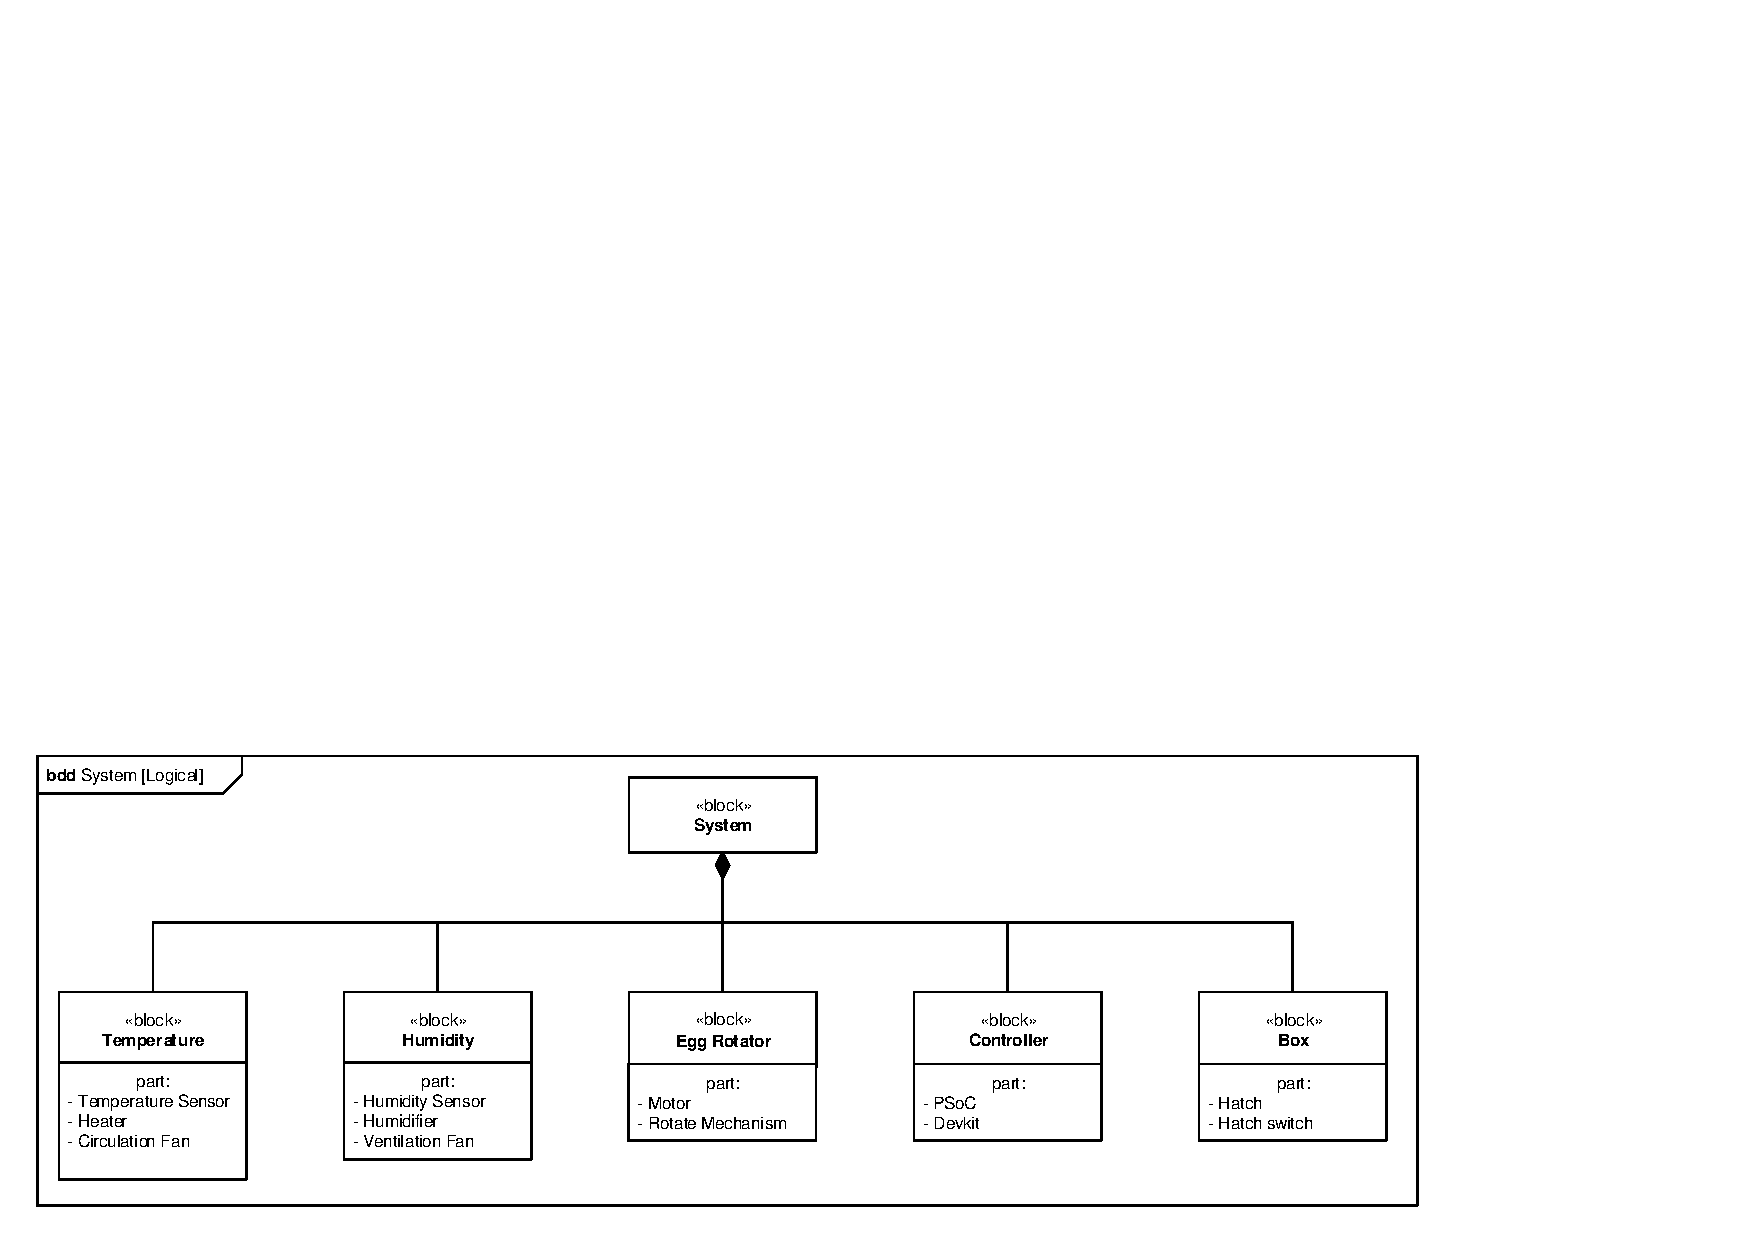
\includegraphics[page=1,width=\linewidth,viewport=08mm 8mm 238mm 80mm]{./2_systemarkitektur/diagrammer/SYSML_Diagrammer_v4.pdf}
\caption[Diagram]{Logical bdd}
\label{fig:SystemStateDiagram}
\end{figure}

\clearpage

\subsection{Physical bdd}

Nedenstående ses et fysisk bdd for systemet, dette diagram er med til at give et overblik over de enkelte fysiske enheder og deres relationer, ligeledes giver dette diagram en hurtig beskrivelse af signalerne som opstår mellem de enkelte fysiske enheder. 

\begin{figure}[H]
\centering
\includegraphics[page=2,width=\linewidth,viewport=8mm 8mm 367mm 185mm]{./2_systemarkitektur/diagrammer/SYSML_Diagrammer_v4.pdf}
\caption[Diagram]{Physical bdd}
\label{fig:SystemStateDiagram}
\end{figure}

\clearpage

\subsection{Internal Block Diagrams}


Figuren herunder viser IBD for hele systemet.
\begin{figure}[H]
\centering
\includegraphics[page=4,width=\linewidth,viewport=8mm 8mm 145mm 58mm]{./2_systemarkitektur/diagrammer/SYSML_Diagrammer_v4.pdf}
\caption[Diagram]{IBD for System}
\label{fig:InternalBlockDiagramFysisk}
\end{figure}


%\begin{flushleft}
Figuren herunder viser IBD for Slave delen af systemet, som er den mest komplekse del af det overordnede system.
%\end{flushleft}
\begin{figure}[H]
\centering
\includegraphics[page=3,width=\linewidth,viewport=8mm 8mm 265mm 212mm]{./2_systemarkitektur/diagrammer/SYSML_Diagrammer_v4.pdf}
\caption[Diagram]{IBD for Slave}
\label{fig:InternalBlockDiagramSlave}
\end{figure}

\clearpage


\subsection{Class Diagram System}

Med udgangspunkt i Usecasen blev der sammen med sekvensdiagrammerne udarbejdet et Klasse diagram. Dette giver overblik over og samler alle funktioner brugt i de to sekvensdiagrammer. Flere af funktionerne har ikke fået angivet retur- og/eller parametre type. Dette er grundet at der mangler at blive taget stilling til disse.

\begin{figure}[H]
\centering
\includegraphics[page=4,width=\linewidth,viewport=7mm 7mm 108mm 68mm]{./2_systemarkitektur/diagrammer/ArkitekturDiagrammer.pdf}
\caption[Diagram]{Class diagram}
\label{fig:SystemStateDiagram}
\end{figure}

\clearpage